% 依固定来源解答页转绘辅助点；只表示题目给定线面关系。
\begin{center}
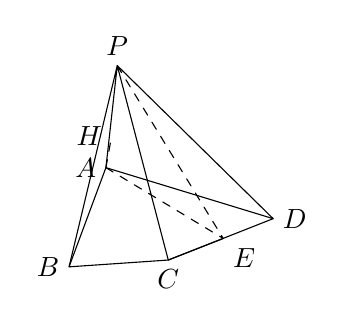
\begin{tikzpicture}[x=0.72cm,y=0.72cm,>=stealth,line cap=round,line join=round]
  \coordinate (B) at (0,0);
  \coordinate (A) at (0.65,1.75);
  \coordinate (C) at (1.75,0.12);
  \coordinate (D) at (3.6,0.85);
  \coordinate (P) at (0.85,3.55);
  \coordinate (E) at (2.72,0.5);
  \coordinate (H) at (0.75,2.3);
  \draw (A)--(D)--(C)--(B)--cycle;
  \draw (P)--(A) (P)--(B) (P)--(C) (P)--(D);
  \draw[dashed] (A)--(E) (P)--(E) (A)--(H);
  \draw (E)--(C);
  \node[left] at (A) {$A$};
  \node[left] at (B) {$B$};
  \node[below] at (C) {$C$};
  \node[right] at (D) {$D$};
  \node[above] at (P) {$P$};
  \node[below right] at (E) {$E$};
  \node[left] at (H) {$H$};
\end{tikzpicture}
\end{center}
